% called by main.tex
%
\chapter{Resultados I: Línea base y ajuste supervisado serializado}
\label{ch::chapter5}

El capítulo~\ref{ch::chapter4} fijó el protocolo que guía la evaluación: representación canónica
en bloques estructurados, pipeline determinista de reconstrucción y un sistema de métricas multinivel
que diferencia validez sintáctica, fidelidad estructural, cobertura semántica y conformidad con el
dominio Kubernetes. Este capítulo aplica ese protocolo a las dos primeras etapas de la comparativa:
la línea base zero-shot y el ajuste fino supervisado con serialización de jerarquía en superficie
(\texttt{serialized\_sft}). El split de test queda reservado para la evaluación conjunta de todas
las arquitecturas al final del trabajo. Todos los resultados presentados aquí corresponden
al split de validación.

Conviene señalar una asimetría de representación antes de interpretar las cifras. La línea base
genera su salida en formato \texttt{blocks\_tsv\_compact\_v1}, que omite la columna
\texttt{line\_index} y la recupera implícitamente del orden de las filas. El SFT serializado
genera en \texttt{blocks\_tsv\_v1}, que incluye \texttt{line\_index} de forma explícita. Ambas
variantes pasan por el mismo parser determinista y el mismo protocolo de evaluación, por lo que
las métricas sobre el YAML reconstruido son comparables entre sí. La diferencia de superficie
es relevante para entender el diseño de cada etapa, pero no distorsiona la comparación de calidad.

%----------------------------------------------------------------------
\section{Línea base zero-shot}
\label{sec:ch5_baseline}
%----------------------------------------------------------------------

Para entender qué aportan las etapas supervisadas, es útil empezar por una pregunta más sencilla:
¿qué puede hacer el modelo base sin ningún ajuste, con una instrucción en lenguaje natural y un
formato de salida explícito en el prompt? Esta configuración se apoya en la capacidad de los modelos de instrucción para seguir especificaciones dadas en lenguaje natural \citep{wei2022scaling, liu2023pretrain}. La respuesta no es trivial a priori.
Qwen2.5-7B-Instruct \citep{qwen2024qwen25} es un modelo de instrucción de propósito general que ha procesado cantidades
significativas de código y configuración YAML durante su preentrenamiento, y el prompt del baseline
describe el formato de bloque esperado con ejemplos concretos. La pregunta relevante no es si el
modelo entiende Kubernetes en algún grado, que probablemente sí, sino si puede mantener la
consistencia jerárquica que exige la reconstrucción determinista del parser para producir
YAML válido de principio a fin.

La Tabla~\ref{tab:ch5_baseline_metrics} recoge las métricas principales del baseline
en el split de validación.

\begin{table}[htbp]
\centering
\caption{Métricas del baseline zero-shot en el split de validación
         (70 muestras totales; 65 con salida estructurada parseable).}
\label{tab:ch5_baseline_metrics}
\begin{tabular}{lc}
\toprule
\textbf{Métrica} & \textbf{Valor} \\
\midrule
Muestras evaluadas             & 65\,/\,70 \\
\texttt{structured\_output\_parse\_success\_rate} & 92{,}86\,\% \\
\texttt{yaml\_parse\_success\_rate}               & 30{,}77\,\% \\
\texttt{average\_level\_mae}                      & 0{,}7896 \\
\texttt{average\_level\_exact\_match\_rate}       & 11{,}31\,\% \\
\texttt{average\_line\_text\_f1}                  & 20{,}86\,\% \\
\texttt{average\_semantic\_key\_f1}               & 27{,}78\,\% \\
\texttt{average\_prompt\_requirement\_f1}         & 22{,}13\,\% \\
\texttt{required\_field\_complete\_sample\_rate}  & 70{,}59\,\% \\
\bottomrule
\end{tabular}
\end{table}

La primera observación que surge es una aparente paradoja: la tasa de parseo estructurado
asciende al 92{,}86\,\%, lo que indica que el modelo sigue el formato de bloque en casi todos
los casos. Sin embargo, solo el 30{,}77\,\% de las muestras produce un YAML válido tras la
reconstrucción con el parser. La Figura~\ref{fig:ch5_baseline_states} desglosa ese resultado
en tres categorías sobre el total de 70 muestras.

Esta diferencia puede resumirse mediante una brecha de parseabilidad entre la superficie estructurada y el YAML reconstruido:

\[
g_{\mathrm{parse}} =
\texttt{structured\_output\_parse\_success\_rate}
-
\texttt{yaml\_parse\_success\_rate}.
\]

En el baseline, esta brecha alcanza \(0{,}9286 - 0{,}3077 = 0{,}6209\), es decir, algo más de 62 puntos porcentuales. El valor refleja que el cuello de botella no está en producir una tabla reconocible, sino en que los niveles generados sean compatibles con una reconstrucción YAML válida.

\begin{figure}[htbp]
\centering
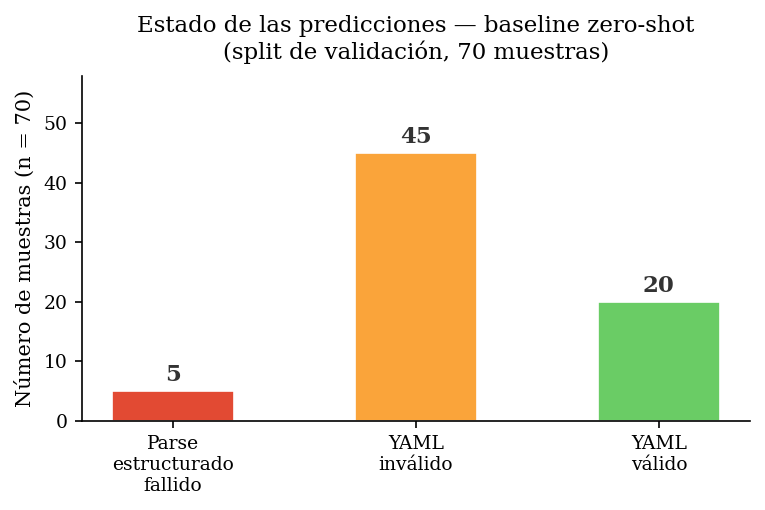
\includegraphics[width=0.68\textwidth]{figures/chapter5/fig5_1_baseline_states.png}
\caption{Estado de las predicciones del baseline zero-shot en el split de validación.
         De las 70 muestras, 65 producen una salida estructurada parseable, pero solo 20 dan
         lugar a un YAML válido tras la reconstrucción determinista. El cuello de botella no
         es el formato de bloque sino la consistencia jerárquica dentro de él.}
\label{fig:ch5_baseline_states}
\end{figure}

La paradoja se disuelve cuando se examina qué falla exactamente. El modelo produce un output
estructurado reconocible, es decir, el bloque TSV se puede parsear. Sin embargo, la asignación de la columna
\texttt{level} es inconsistente a medida que avanza la secuencia generada. En particular, los
desajustes acumulativos en la indentación a lo largo de varias decenas de tokens introducen
errores que el parser no puede recuperar: el resultado es un \texttt{ScannerError} o
\texttt{ParserError} en el momento de reconstruir el árbol YAML. El
\texttt{average\_level\_mae} de 0{,}79 lo cuantifica: en promedio, el nivel predicho se aleja
casi una unidad completa de sangría del nivel correcto. Para una estructura YAML donde cada
unidad representa dos espacios de indentación, ese margen es suficiente para romper
la coherencia del árbol.

Las métricas semánticas confirman el mismo límite desde otra perspectiva. Un
\texttt{semantic\_key\_f1} del 27{,}78\,\% indica que poco más de una cuarta parte de las
claves semánticas esperadas aparecen en la predicción. El
\texttt{average\_prompt\_requirement\_f1} del 22{,}13\,\% añade que los requisitos explícitos
del prompt (el tipo de recurso solicitado, el nombre, el número de réplicas, el namespace, etc.)
se satisfacen en apenas una de cada cinco muestras. Y solo el 70{,}59\,\% de las muestras
produce recursos con todos los campos obligatorios presentes. En conjunto, el baseline refleja
que el modelo reconoce el dominio a nivel de superficie, y produce un output con aspecto de
manifiesto. Sin embargo, carece tanto del control jerárquico como de la cobertura semántica que
necesita el parser para que ese manifiesto sea estructuralmente válido y funcionalmente completo.
Ese es el suelo empírico a partir del cual operan las etapas supervisadas.


%----------------------------------------------------------------------
\section{\texttt{serialized\_sft}: ajuste con jerarquía en superficie}
\label{sec:ch5_sft}
%----------------------------------------------------------------------

El \texttt{serialized\_sft} parte de la hipótesis de que el problema del baseline admite una
solución mediante ajuste fino supervisado con LoRA \citep{hu2021lora, dettmers2023qlora, wu2025sft}: si el modelo aprende a generar secuencias
de bloques bien formadas en el formato \texttt{blocks\_tsv\_v1}, el parser determinista debería
poder reconstruir YAML válido en casi todos los casos. La jerarquía no se predice mediante
ningún mecanismo estructural separado; se serializa en la superficie textual como una columna
más del TSV. La pregunta de fondo es si esa codificación implícita es suficiente para resolver
el problema de consistencia de niveles que el zero-shot no puede superar.
En la arquitectura del trabajo, esta variante actúa como modelo de control: su función es
establecer hasta dónde llega la serialización de jerarquía en superficie antes de comparar
con el \texttt{two\_head\_sft}, donde la predicción de \texttt{level} se desacopla de la
generación de contenido de línea mediante una cabeza estructural dedicada.

La Tabla~\ref{tab:ch5_comparison} presenta la comparativa completa entre el baseline y el SFT
serializado en el split de validación. Para cada métrica \(m\), la diferencia se calcula como:

\[
\Delta_m = m(\texttt{serialized\_sft}) - m(\texttt{baseline}).
\]

En las métricas donde valores mayores son mejores, un \(\Delta_m\) positivo indica mejora; en el caso de \texttt{average\_level\_mae}, la mejora aparece como una diferencia negativa porque se trata de un error.

\begin{table}[htbp]
\centering
\caption{Comparativa de métricas entre el baseline zero-shot y \texttt{serialized\_sft}
         en el split de validación. $\Delta$ indica la diferencia en puntos porcentuales
         (métricas de tasa) o en unidades absolutas (\texttt{level\_mae}).}
\label{tab:ch5_comparison}
\begin{tabular}{lccc}
\toprule
\textbf{Métrica} & \textbf{Baseline} & \textbf{\texttt{serialized\_sft}} & $\boldsymbol{\Delta}$ \\
\midrule
Muestras evaluadas
    & 65\,/\,70 & 70\,/\,70 & --- \\
\texttt{structured\_output\_parse\_success\_rate}
    & 92{,}86\,\% & 100{,}00\,\% & \textbf{+7{,}14} \\
\texttt{yaml\_parse\_success\_rate}
    & 30{,}77\,\% & 98{,}57\,\% & \textbf{+67{,}80} \\
\texttt{average\_level\_mae}
    & 0{,}7896 & 0{,}2723 & $\mathbf{-0{,}517}$ \\
\texttt{average\_level\_exact\_match\_rate}
    & 11{,}31\,\% & 75{,}78\,\% & \textbf{+64{,}47} \\
\texttt{average\_line\_text\_f1}
    & 20{,}86\,\% & 82{,}06\,\% & \textbf{+61{,}20} \\
\texttt{average\_semantic\_key\_f1}
    & 27{,}78\,\% & 95{,}52\,\% & \textbf{+67{,}74} \\
\texttt{average\_prompt\_requirement\_f1}
    & 22{,}13\,\% & 85{,}31\,\% & \textbf{+63{,}18} \\
\texttt{required\_field\_complete\_sample\_rate}
    & 70{,}59\,\% & 100{,}00\,\% & \textbf{+29{,}41} \\
\bottomrule
\end{tabular}
\end{table}

El salto es consistente en todas las métricas: ninguna empeora y varias mejoran más de 60 puntos porcentuales. La tasa de parseo YAML pasa de 30{,}77\,\% a
98{,}57\,\%: el problema de consistencia estructural que dominaba el baseline queda resuelto en
casi todos los casos. El \texttt{average\_level\_mae} cae de 0{,}79 a 0{,}27, lo que implica
que el error promedio de indentación por línea se reduce a poco más de un cuarto de unidad. Las
métricas semánticas reflejan el mismo patrón: \texttt{semantic\_key\_f1} pasa de 27{,}78\,\%
a 95{,}52\,\%, y los campos obligatorios, que el baseline completaba en apenas el 70{,}59\,\%
de las muestras, aparecen completos en el 100\,\% de los manifiestos generados por el SFT. La
predicción de nivel exacto (\texttt{level\_exact\_match\_rate}) mejora de 11{,}31\,\% a
75{,}78\,\%, lo que confirma que, en esta primera formulación, la serialización superficial de la jerarquía es suficiente
para que el modelo aprenda a asignar indentaciones correctas en la gran mayoría de las líneas.

La Figura~\ref{fig:ch5_training_loss} muestra la evolución de la pérdida durante las
tres épocas de entrenamiento.

\begin{figure}[htbp]
\centering
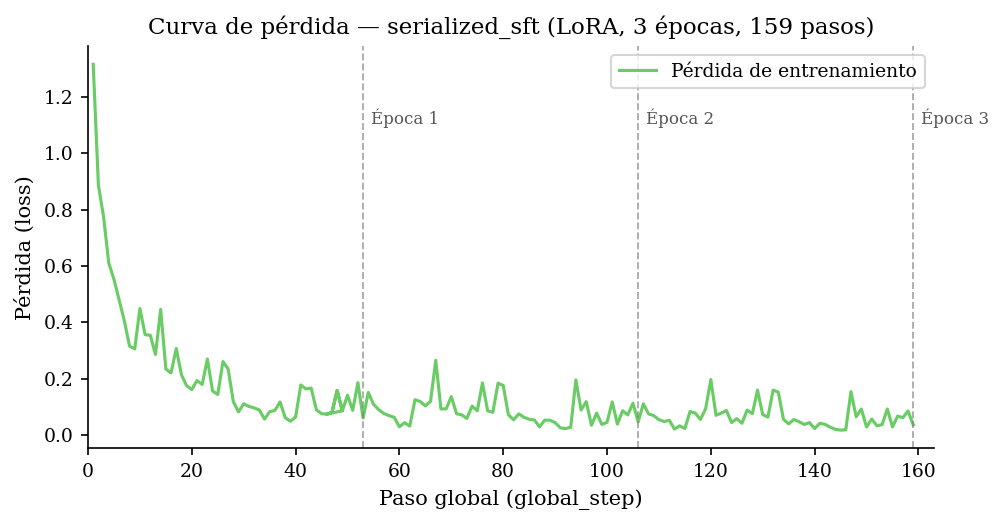
\includegraphics[width=0.88\textwidth]{figures/chapter5/fig5_2_training_loss.png}
\caption{Curva de pérdida de entrenamiento del \texttt{serialized\_sft}
         (LoRA, 3 épocas, 159 pasos globales, 424 muestras de entrenamiento efectivas (426 nominales, 2 omitidas por OOM)).
         La pérdida desciende de 1{,}32 en el primer paso a valores inferiores a 0{,}2 al final
         de la primera época. Las épocas segunda y tercera refinan los casos más complejos,
         con valores de pérdida entre 0{,}03 y 0{,}09.}
\label{fig:ch5_training_loss}
\end{figure}

La convergencia es rápida, especialmente en los primeros pasos. La pérdida cae de 1{,}32 a
valores inferiores a 0{,}2 antes del fin de la primera época (paso~53), lo que sugiere que el
modelo asimila la estructura del formato \texttt{blocks\_tsv\_v1} con pocas iteraciones. Las
Las épocas segunda y tercera refinan los casos residuales ---posiblemente manifiestos con
mayor profundidad jerárquica o con múltiples documentos, aunque el log de entrenamiento no
desglosa la pérdida por muestra--- sin descensos tan abruptos, sino con una reducción
progresiva y ruidosa que es esperable en un entrenamiento con batch efectivo pequeño. Cabe
señalar que durante el proceso se omitieron dos microbatches por recuperación de OOM: los
ejemplos \texttt{q229::question} y \texttt{q229::question\_simplified}, que superan los 3100
caracteres de prompt y objetivo combinados. La omisión está registrada en
\texttt{oom\_skipped\_batches.jsonl}; el conjunto de entrenamiento efectivo es de 424 muestras.

La Figura~\ref{fig:ch5_metrics_comparison} resume el salto en las cuatro métricas principales.

\begin{figure}[htbp]
\centering
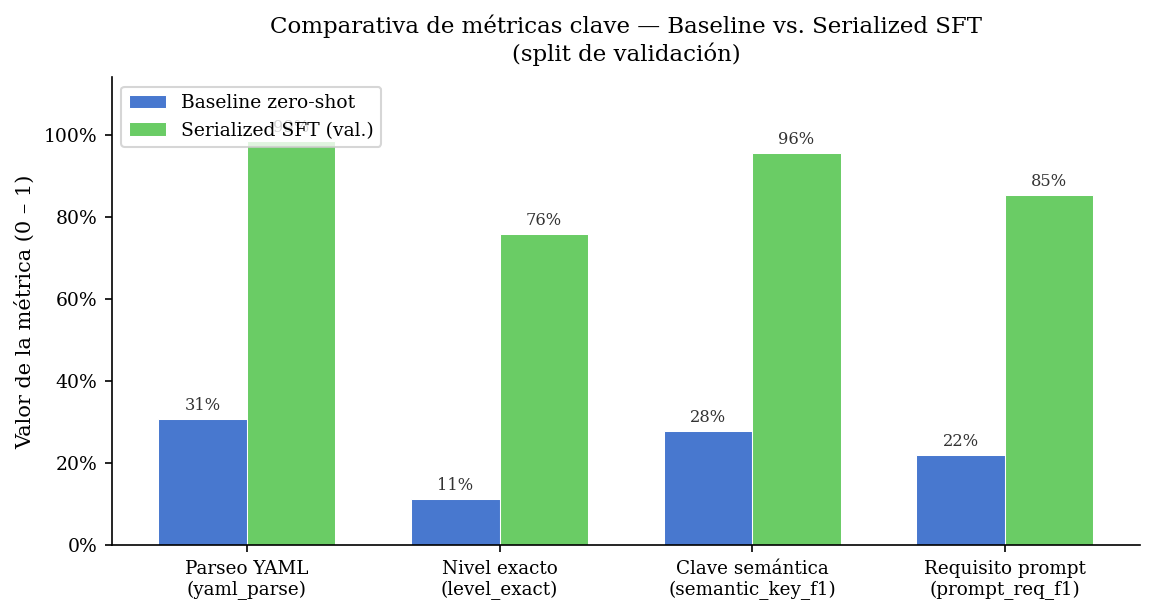
\includegraphics[width=0.92\textwidth]{figures/chapter5/fig5_3_metrics_comparison.png}
\caption{Comparativa de métricas clave entre el baseline zero-shot y el \texttt{serialized\_sft}
         en el split de validación. El salto de 31\,\% a 99\,\% en parseo YAML y de 28\,\%
         a 96\,\% en clave semántica muestra que el SFT resuelve de forma simultánea el
         problema estructural y el de cobertura semántica. La predicción de nivel exacto mejora
         de 11\,\% a 76\,\%, confirmando que la serialización implícita de jerarquía es
         suficiente para aprender indentaciones correctas.}
\label{fig:ch5_metrics_comparison}
\end{figure}

A pesar de ese avance, la compuerta de validez de dominio Kubernetes descubre un cuello de
botella que la supervisión pura no resuelve: solo el 14{,}29\,\% de las muestras superan la
compuerta completa. La Tabla~\ref{tab:ch5_domain_levels} desglosa la tasa de superación por
nivel de compuerta.

\begin{table}[htbp]
\centering
\caption{Tasa de superación de la compuerta de validez de dominio Kubernetes por nivel
         para el \texttt{serialized\_sft} en el split de validación (70 muestras).
         Los niveles son acumulativos: superar el nivel $k$ implica haber superado los
         niveles $0,\ldots,k-1$. La compuerta final corresponde al nivel 5.}
\label{tab:ch5_domain_levels}
\begin{tabular}{clc}
\toprule
\textbf{Nivel} & \textbf{Criterio evaluado} & \textbf{Tasa de paso} \\
\midrule
0 & Identidad básica: \texttt{apiVersion} y \texttt{kind} reconocibles & 98{,}57\,\% \\
1 & Metadatos mínimos: \texttt{metadata.name} presente               & 98{,}57\,\% \\
2 & Campos obligatorios según el \texttt{kind}                        & 97{,}14\,\% \\
3 & Estructura \texttt{spec} completa (contenedores, puertos)         & 91{,}43\,\% \\
4 & Consistencia selector--template y coherencia de volúmenes         & 90{,}00\,\% \\
5 & Prácticas de seguridad (límites de recursos, contexto, imagen)    & \textbf{14{,}29\,\%} \\
\midrule
\multicolumn{2}{l}{\texttt{kubernetes\_domain\_gate\_pass\_rate} (compuerta final)} & 14{,}29\,\% \\
\bottomrule
\end{tabular}
\end{table}

Los niveles 0 a 4 se superan con tasas del 90\,\% al 99\,\%, lo que confirma que el SFT
gestiona bien los aspectos estructurales y semánticos básicos de los manifiestos. El colapso
se produce en el nivel 5, que evalúa prácticas de seguridad: especificación de límites de
recursos de CPU y memoria, configuración del contexto de seguridad del contenedor
(\texttt{runAsNonRoot}, \texttt{readOnlyRootFilesystem}) y uso de etiquetas de imagen no
flotantes. En ese nivel la tasa cae al 14{,}29\,\%. El nivel de validez de dominio promedio
por muestra es de 3{,}9, coherente con el perfil observado: la mayoría de los manifiestos
alcanzan el nivel 4 y fallan en el umbral de seguridad.

La magnitud de ese cuello de botella puede expresarse como la caída entre la última compuerta semántica superada de forma mayoritaria y la compuerta de seguridad:

\[
\mathrm{drop}_5 = \mathrm{pass}_4 - \mathrm{pass}_5
= 0{,}9000 - 0{,}1429 = 0{,}7571.
\]

Esta caída de 75{,}71 puntos porcentuales resume por qué el problema residual no es ya principalmente sintáctico ni estructural, sino de alineación con criterios de calidad estática.

Este resultado no implica que la representación serializada sea incorrecta ni insuficiente
para capturar jerarquía. Lo que ocurre es distinto: el SFT ha aprendido a generar manifiestos
estructuralmente correctos y funcionalmente coherentes, pero ha aprendido también a reproducir
los patrones que predominan en los datos de entrenamiento, que probablemente incluyen
manifiestos de ejemplo o de desarrollo sin restricciones de seguridad, un patrón coherente con estudios empíricos sobre misconfigurations y smells de seguridad en Kubernetes \citep{rahman2023securityk8s, zhang2024generativeSmells}. La compuerta de nivel 5
detecta precisamente esa ausencia sistemática. No es un fallo de formato sino de alineación
con las prácticas que el evaluador de dominio considera obligatorias.

Un experimento adicional permite precisar esa afirmación. Se evaluó un run de entrenamiento
independiente de una sola época con configuración idéntica
(\texttt{serialized-sft-a-v1-1epoch-20260507-1528}), cuyo checkpoint final (paso~53)
corresponde al cierre de la primera época; el checkpoint equivalente del run de tres épocas
fue descartado por la política de retención de checkpoints. El objetivo es desagregar cuánto
del salto total produce cada fase de entrenamiento. Con una sola época el modelo ya alcanza una tasa de
parseo YAML del 90\,\%, un \texttt{semantic\_key\_f1} del 85{,}83\,\% y un MAE de nivel de
0{,}297. Las dos épocas restantes refinan esas cifras de forma apreciable: el parseo YAML sube
hasta el 98{,}57\,\%, el \texttt{semantic\_key\_f1} escala al 95{,}52\,\% y el MAE de nivel
desciende a 0{,}272. Lo que no cambia en absoluto es la tasa de superación de la compuerta de
nivel~5: 14{,}29\,\% al final de la primera época y exactamente 14{,}29\,\% al final de la
tercera. Más iteraciones sobre los mismos datos refinan la calidad estructural y semántica del
modelo, pero no acercan ni un punto porcentual al techo impuesto por los requisitos de seguridad.
Esa invarianza es el argumento empírico más directo contra una lectura de insuficiencia de
entrenamiento: el cuello de botella no está en cuántas veces ve el modelo los datos, sino en
qué señal contienen esos datos. La Tabla~\ref{tab:ch5_epoch_ablation} recoge la comparativa
completa entre ambos checkpoints.

\begin{table}[htbp]
\centering
\caption{Comparativa de métricas entre el run de 1~época (paso~53) y el modelo final
         de 3~épocas (paso~159) del \texttt{serialized\_sft} en el split de validación
         (70~muestras). $\Delta$ indica la diferencia en puntos porcentuales o en unidades
         absolutas (\texttt{level\_mae}).}
\label{tab:ch5_epoch_ablation}
\begin{tabular}{lccc}
\toprule
\textbf{Métrica} & \textbf{1 época} & \textbf{3 épocas} & $\boldsymbol{\Delta}$ \\
\midrule
\texttt{yaml\_parse\_success\_rate}
    & 90{,}00\,\% & 98{,}57\,\% & \textbf{+8{,}57} \\
\texttt{average\_level\_mae}
    & 0{,}2974 & 0{,}2723 & $\mathbf{-0{,}025}$ \\
\texttt{average\_level\_exact\_match\_rate}
    & 66{,}44\,\% & 75{,}78\,\% & \textbf{+9{,}34} \\
\texttt{average\_line\_text\_f1}
    & 73{,}37\,\% & 82{,}06\,\% & \textbf{+8{,}69} \\
\texttt{average\_semantic\_key\_f1}
    & 85{,}83\,\% & 95{,}52\,\% & \textbf{+9{,}69} \\
\texttt{average\_prompt\_requirement\_f1}
    & 77{,}16\,\% & 85{,}31\,\% & \textbf{+8{,}15} \\
\texttt{required\_field\_complete\_sample\_rate}
    & 98{,}41\,\% & 100{,}00\,\% & \textbf{+1{,}59} \\
\texttt{kubernetes\_domain\_gate\_pass\_rate}
    & 14{,}29\,\% & 14{,}29\,\% & \textbf{0{,}00} \\
\bottomrule
\end{tabular}
\end{table}


%----------------------------------------------------------------------
\section{Análisis de errores del SFT serializado}
\label{sec:ch5_sft_errors}
%----------------------------------------------------------------------

Confrontar el perfil de errores del baseline con el del SFT resulta revelador porque los dos
fallan de formas cualitativamente distintas. El baseline fallaba principalmente por
inconsistencia estructural: niveles de indentación incorrectos, subtrees truncados, confusión
entre mappings y listas en posiciones profundas del árbol YAML. El SFT serializado elimina
casi por completo ese tipo de error. Lo que permanece es diferente en naturaleza.

La Tabla~\ref{tab:ch5_error_profile} muestra los conteos de errores de dominio detectados por
el evaluador automático en el split de validación, acumulados sobre todos los recursos generados.

\begin{table}[htbp]
\centering
\caption{Perfil de errores de dominio del \texttt{serialized\_sft} en el split de validación
         (70 muestras). Los conteos son acumulados sobre todos los recursos generados; una
         muestra puede contener varios recursos y contribuir con múltiples instancias
         del mismo tipo de error.}
\label{tab:ch5_error_profile}
\begin{tabular}{p{0.38\textwidth}p{0.29\textwidth}rp{0.12\textwidth}}
\toprule
\textbf{Tipo de error} & \textbf{Descripción} & \textbf{Inst.} & \textbf{Categoría} \\
\midrule
\texttt{missing\_resource\_requirement}
    & Sin límites de CPU/memoria & 261 & Seguridad \\
\texttt{missing\_run\_as\_non\_root}
    & Contenedor ejecutable como root & 71 & Seguridad \\
\texttt{missing\_read\_only\_root\_filesystem}
    & FS raíz no read-only & 71 & Seguridad \\
\texttt{latest\_image\_tag}
    & Imagen con etiqueta \texttt{:latest} & 67 & Seguridad \\
\texttt{volume\_mount\_without\_volume}
    & Volumen montado sin declaración & 5 & Semántica \\
\texttt{service\_selector\_without\_workload}
    & Selector sin workload asociado & 1 & Semántica \\
\texttt{yaml\_parse}
    & Fallo residual de parseo YAML & 1 & Estructura \\
\texttt{kubernetes\_identity}
    & Identidad de recurso inválida & 1 & Estructura \\
\midrule
\multicolumn{2}{l}{Antipatrones de seguridad (subtotal)} & 470 & \\
\multicolumn{2}{l}{Errores estructurales y semánticos (subtotal)} & 8 & \\
\bottomrule
\end{tabular}
\end{table}

La distribución es llamativa por su asimetría. Los cuatro antipatrones de seguridad acumulan
470 instancias frente a 8 instancias de errores estructurales o de semántica local. En términos relativos, la proporción de errores atribuibles a seguridad dentro del perfil medido es:

\[
\rho_{\mathrm{seguridad}} =
\frac{470}{470 + 8}
= 0{,}983.
\]

Es decir, el 98{,}3\,\% de las instancias registradas en este perfil pertenecen a la misma familia de fallo.
La Figura~\ref{fig:ch5_domain_errors} lo visualiza.

\begin{figure}[htbp]
\centering
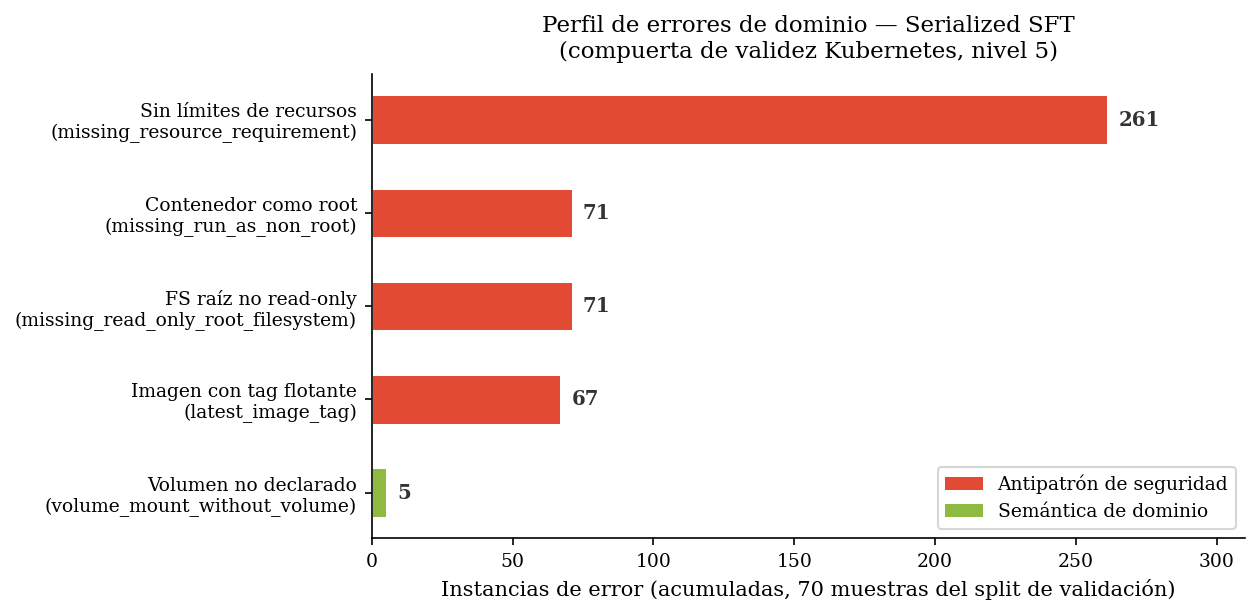
\includegraphics[width=0.92\textwidth]{figures/chapter5/fig5_4_domain_errors.png}
\caption{Distribución de errores de dominio del \texttt{serialized\_sft} en el split
         de validación. Los cuatro antipatrones de seguridad (rojo) acumulan 470 instancias;
         los errores de semántica de dominio (verde) se limitan a 7 instancias. El perfil
         refleja que el SFT ha resuelto el problema estructural pero ha heredado los patrones
         inseguros presentes en los datos de entrenamiento.}
\label{fig:ch5_domain_errors}
\end{figure}

Este perfil tiene una interpretación concreta. El SFT ha aprendido a reproducir la superficie
de los manifiestos Kubernetes con alta fidelidad, incluyendo los patrones de los ejemplos de
entrenamiento. Si esos ejemplos no especifican límites de recursos, no configuran
\texttt{runAsNonRoot} ni \texttt{readOnlyRootFilesystem}, y emplean la etiqueta \texttt{:latest}
en las imágenes, el modelo aprende a hacer lo mismo. La estructura resultante es correcta, los
campos requeridos están presentes y la jerarquía es coherente; pero las restricciones de seguridad
que un entorno de producción exigiría están sistemáticamente ausentes. No es un límite de la
representación serializada: es un límite de lo que la supervisión sola puede transmitir.

Los errores estructurales residuales merecen un comentario separado. Las 5 instancias de
\texttt{volume\_mount\_without\_volume} representan un error de coherencia semántica local: el
modelo declara una referencia a un volumen en la spec del contenedor, pero no incluye la
declaración correspondiente en la sección \texttt{volumes} del pod. Se trata de un problema de
alcance contextual ---el modelo no conecta las dos partes de la especificación--- y no de
indentación ni de parseo. El único caso de \texttt{service\_selector\_without\_workload} y el
único fallo residual de parseo YAML son instancias aisladas sin patrón sistemático.

El análisis de errores del SFT serializado señala, por tanto, un cambio cualitativo respecto
al baseline. Antes de la supervisión, el límite era estructural: el modelo no mantenía la
jerarquía. Después de la supervisión, el límite es de alineación: el modelo no incorpora las
prácticas de seguridad que el evaluador de dominio requiere. Esa distinción importa en dos direcciones. Por un lado, el gap de seguridad muestra que la
supervisión pura sobre los datos actuales no es suficiente para adquirir las prácticas de
dominio que el evaluador requiere; la señal que falta no es de cantidad sino de preferencia,
y eso es lo que abre la puerta a una fase de alineación basada en DPO \citep{rafailov2023dpo, xu2024dpoPpo}. Por otro lado, la
pregunta estructural que motiva el diseño del trabajo sigue abierta: el capítulo siguiente
evalúa si una cabeza de predicción explícita de \texttt{level} ---en lugar de su serialización
en la superficie del texto--- produce mejoras adicionales en la calidad jerárquica que la
variante serializada no alcanza. Ambas líneas de continuidad arrancan del perfil de errores
documentado aquí.
